%%%%%%%%%%%%%%%%%%%%%%%%%%%%%%%%%%%%%%%%%%%%%%%%%%%%%%%%%%%%%%%%%%%%%%%%%%%%%%%%%%%%%%%%%%%%%%%%%%%%%%%%%%%%%%%%%%%%%%%%%%%%%%%%%%%%%%%%%%%%%%%%%%%%%%%%%%%
% This is just an example/guide for you to refer to when submitting manuscripts to Frontiers, it is not mandatory to use frontiers.cls nor frontiers.tex  %
% This will only generate the Manuscript, the final article will be typeset by Frontier after acceptance.                                                 %
%                                                                                                                                                         %
% When submitting your files, remember to upload this *tex file, the pdf generated with it, and all the figures.
%%%%%%%%%%%%%%%%%%%%%%%%%%%%%%%%%%%%%%%%%%%%%%%%%%%%%%%%%%%%%%%%%%%%%%%%%%%%%%%%%%%%%%%%%%%%%%%%%%%%%%%%%%%%%%%%%%%%%%%%%%%%%%%%%%%%%%%%%%%%%%%%%%%%%%%%%%%

%%% Version 2.1 Generated 2013/11/27 %%%
%%% You will need to have the following packages installed: datetime, fmtcount, etoolbox, fcprefix, which are normally inlcuded in WinEdt. %%%
%%% In http://www.ctan.org/ you can find the packages and how to install them, if necessary. %%%

\documentclass{frontiersSCNS} % for Science articles

%\setcitestyle{square}
\usepackage{url,lineno}
\usepackage[utf8]{inputenc}
\usepackage{listings}
\linenumbers

\lstdefinestyle{display}{
  basicstyle=\ttfamily\footnotesize,
}

%%%%%%%%%%%%%%%%%%%%%%%%%%%%%%%%%%%%%%%%%
% PR start ******************************

% double spacing for editorial work
%\usepackage{setspace}
%\doublespacing

% new commands
\newcommand{\pr}[1]{[\textcolor{YellowOrange}{PR: #1}]}

% remarks:
% Images:
% Image size for figures: 180 mm width with 900 - 1200 dpi.
% 180 mm and 1200 dpi ==> 8504 pixel
% 85 mm and 1200 dpi ==> 4016
%
% maybe better: safe as pdf and then use http://tex.stackexchange.com/questions/20883/how-to-convert-pdf-to-eps
% to convert to eps (saving it from inkscape directly as eps doesn't work as
% the result is pixeled)


% PR stop ******************************
%%%%%%%%%%%%%%%%%%%%%%%%%%%%%%%%%%%%%%%%


% Leave a blank line between paragraphs in stead of using \\

\copyrightyear{}
\pubyear{}

\def\journal{Neuroinformatics}%%% write here for which journal %%%
\def\DOI{}
\def\articleType{Technology Report}
\def\keyFont{\fontsize{8}{11}\helveticabold }
\def\firstAuthorLast{Rautenberg {et~al.}} %use et al only if is more than 1 author
\def\Authors{
Philipp L. Rautenberg\,$^{1,2*}$,
Alvaro Tejero-Cantero\,$^{3}$,
Ajayrama Kumaraswamy\,$^{1}$,
Christoph Doblander\,$^{4}$,
Mohammad Reza Norouzian\,$^{4}$,
Kazuki Kai\,$^{5}$,
Hans-Arno Jacobsen\,$^{4}$,
Hiroyuki Ai\,$^{5}$,
Thomas Wachtler\,$^{1}$,
and Hidetoshi Ikeno\,$^6$}
% Affiliations should be keyed to the author's name with superscript numbers and be listed as follows: Laboratory, Institute, Department, Organization, City, State abbreviation (USA, Canada, Australia), and Country (without detailed address information such as city zip codes or street names).
% If one of the authors has a change of address, list the new address below the correspondence details using a superscript symbol and use the same symbol to indicate the author in the author list.
\def\Address{$^{1}$Department of Biology II, Ludwig-Maximilians-Universität, Germany\\
$^{2}$Max Planck Digital Library, München, Germany\\
$^{3}$MRC ANU, Department of Pharmacology, University of Oxford, United Kingdom\\
$^{4}$Department of Informatics, Technische Universität München, Germany\\
$^{5}$Department of Earth System Science, Fukuoka University, Japan\\
$^{6}$School of Human Science and Environment, University of Hyogo, Japan
}
% The Corresponding Author should be marked with an asterisk
% Provide the exact contact address (this time including street name and city zip code) and email of the corresponding author
\def\corrAuthor{Philipp L. Rautenberg}
\def\corrAddress{Department of Biology II, Ludwig-Maximilians-Universität, Germany}
\def\corrEmail{rautenberg@biologie.uni-muenchen.de}

% \color{FrontiersColor} Is the color used in the Journal name, in the title, and the names of the sections.


\begin{document}
\onecolumn
\firstpage{1}

\title[NeuronDepot – Keeping your colleagues in sync]{NeuronDepot – Keeping your colleagues in sync by combining modern cloud storage services, local the file system, and user-friendly web techniques}
\author[\firstAuthorLast ]{\Authors}
\address{}
\correspondance{}
\extraAuth{}% If there are more than 1 corresponding author, comment this line and uncomment the next one.
%\extraAuth{corresponding Author2 \\ Laboratory X2, Institute X2, Department X2, Organization X2, Street X2, City X2 , State XX2 (only USA, Canada and Australia), Zip Code2, X2 Country X2, email2@uni2.edu}
\topic{Recent advances and the future generation of neuroinformatics infrastructure}% If your article is part of a Research Topic, please indicate here which.

\maketitle

%%%%%%%%%%%%%%%%%%%%%%%%%%%%%%%%%%%%%%%%%%%%%%%%%%%%%%%%%%%%%%%%%%%%%%%%%%%%%%%%%%%%%%%%%%%%%%%%%%%%%%%%%%%%%%%%%%%%%%%%%%%%%%%%%%%%%%%%%%%%%%%%%%%%%%%%%%%%%%%%%%%%%%%%%%%%%%%%%%%%%%%%%%%%%%%%%%%%%%%%%%%%%%%%%%%%%%%%%%%%%%%%%%%%%%%
%%% The sections below are for reference only.
%%%
%%% For Original Research Articles, Clinical Trial Articles, and Technology Reports the section headings should be those appropriate for your field and the research itself. It is recommended to organize your manuscript in the
%%% following sections or their equivalents for your field:
%%% Abstract, Introduction, Material and Methods, Results, and Discussion.
%%% Please note that the Material and Methods section can be placed in any of the following ways: before Results, before Discussion or after Discussion.
%%%
%%%For information about Clinical Trial Registration, please go to http://www.frontiersin.org/about/AuthorGuidelines#ClinicalTrialRegistration
%%%
%%% For Clinical Case Studies the following sections are mandatory: Abstract, Introduction, Background, Discussion, and Concluding Remarks.
%%%
%%% For all other article types there are no mandatory sections.
%%%%%%%%%%%%%%%%%%%%%%%%%%%%%%%%%%%%%%%%%%%%%%%%%%%%%%%%%%%%%%%%%%%%%%%%%%%%%%%%%%%%%%%%%%%%%%%%%%%%%%%%%%%%%%%%%%%%%%%%%%%%%%%%%%%%%%%%%%%%%%%%%%%%%%%%%%%%%%%%%%%%%%%%%%%%%%%%%%%%%%%%%%%%%%%%%%%%%%%%%%%%%%%%%%%%%%%%%%%%%%%%%%%%%%%

\begin{abstract}

\section{
We report here (1) a novel approach to data sharing between collaborating
scientists that brings together filesystem tools and the cloud, (2) a pilot
open-source implementation, called NeuronDepot, and (3) an exemplary application
of the software to a demanding use case in the neurosciences, the GinJang
project. The main drivers for our approach are to provide collaborations with a
transparent, automated data flow and shield scientists from having to learn new
tools or data structuring paradigms. With minimum overhead (one-time data
assignment from the originator) this approach makes experimental and modelling
data available across the collaboration and cloud-ready, opening up the data to
the advantages in software updates, and hardware scalability associated with
elastic cloud computing. We provide a pilot implementation that relies on
existing synchronization services and is usable from all devices via a reactive
web interface. We are motivating our pilot solution solving the practical
problems of the GinJang project, a collaboration of three universities across
eight time zones with a complex workflow encompassing data from
electrophysiological recordings, imaging, morphological reconstructions, and
simulations.
}

\tiny
 \keyFont{ \section{Keywords:} Morphology, Electrophysiology, Imaging, Data
 Management, Neuroinformatics, cloud services} %All article types: you may provide up to 8 keywords; at least 5 are mandatory.
\end{abstract}

%%%%%%%%%%%%%%
% Introduction
%%%%%%%%%%%%%%
%\twocolumn
\section{Introduction}
Science today deals with a “data deluge” derived from the widespread use of
high-throughput sensors in experiments and the ever more complex simulations
afforded by increased computational power. Both measured and simulated data
need to be stored in raw form, preprocessed, contextualized with metadata,
organized to facilitate queries and then analyzed to produce scientific
statements. Ideally, peer-reviewed data should also be available for
replication and reanalysis to test new hypotheses as knowledge progresses.

In addition to these single-lab data management needs, the multidisciplinary
character of many of the questions addressed and their complexity benefit from
the coordinated effort of geographically distributed specialists. The need for
collaboration is particularly acute in neuroscience, an inherently multilevel
enterprise that tackles questions spanning disparate levels of organization
(genes, neurons, circuits, behaviour...) with a variety of methods (sequencing,
anatomy, electrophysiology, computer simulations...). Thus, a collaboration
such as the GinJang project introduced below, supports the scientists.

One particularly problematic aspect of the workflow concerns thus the sharing
across labs of highly structured and voluminous data. Because often pieces of
the workflow are interdependent, a further step of the local work depending on
another operation that is remotely carried out, the process should be as
automatic and as fast as possible. For example analysis results can inform
further experimental data collection, whereupon it is clearly of advantage that
they are made available as they are produced.

Existent proposals to alleviate the data management overhead frequently require
scientists to relinquish their local processing workflow in order to be able to
offer distributed access for collaborators to participate in the project. We
propose here a novel approach which integrates seamlessly the prevalent
filesystem-based acquisition, munging, analysis and publication workflows by
leveraging proven cloud synchronization technology. Our implementation of this
approach, called NeuronDepot enables researchers to continue interacting with
the scientific project database through the filesystem and at the same time
opens up the data for analysis in cloud-based web applications. In this way
NeuronDepot exploits the existing substantial investment in development,
acquisition and training in local applications, with their mature and rich
interfaces and local access to data, and, at the same time, the advantages of
upcoming cloud-based software with its platform independence, managed updates
and transparent scalability. We illustrate the approach with a NeuronDepot
deployment tailored to the specific needs of the GinJang project
[http://projects.g-node.org/ginjang/], a demanding use case that combines data
from electrophysiological recordings, imaging, morphological reconstructions,
and simulations.

We intend for our approach to serve as an example of a gradual path towards the
availability of well marked-up scientific data in the cloud. By offering new
functionality in a way compatible with existing services, tools, training, and
working environments the costs of data sharing in a collaboration are brought
down to a minimum while the accessibility of research assets is future-proofed.

Compared to other data-intensive research disciplines in life sciences such as
genomics and proteomics \citep{Gelbart1997, Stoesser1997, DeSchutter2008},
neurosciences lag behind regarding the use of databases for the organization
and exchange of data. Only recently attempts have started to integrate
neuroscience databases \citep{Amari2002, Gupta2008}, and so far the focus has
been mostly placed on anatomical data. In the domain of neurophysiology, one of
the first public databases for electrophysiological data was the
neurodatabase.org project (\url{http://neurodatabase.org}). In this project, an
elaborate data model and format along with a query protocol for the exchange of
neurophysiological data were developed. The data, typically obtained from
publications is made available with extensive metadata and provided in a
standard format developed in the project.

The CRCNS site (\url{http://crcns.org}) hosts electrophysiological data that have been
specifically selected by contributing labs for the purpose of making the data
available to the public. Typically, these data are from studies that have been
published and they may be used for further investigations after they have
served their primary purpose. Data format and documentation are different for
each dataset.

The CARMEN project (\url{http://www.carmen.org.uk}) provides a platform for data analysis
and data exchange where the owner of the data can keep the data private, or can
make the data available to selected users or the public. The platform also
provides services for data analysis. During file upload, the user has the
option to enter metadata describing the experiment in which the data were
recorded. 

The German Neuroinformatics Node (G-Node) provides a platform for data
organization and data sharing of neurophysiological data
(\url{portal.g-node.org/data}). Users can upload, organize, and annotate data, and
make them accessible to other users or the public. Data conversion functions
are provided. Data annotation follows a flexible schema \citep{Grewe2011} so
that any metadata necessary can be entered. This platform is currently being
extended with an API for fine-grained data access through common languages like
Python or Matlab, which will provide a framework that scientists can use to
manage and access directly from their local data workflow environment.
Recently, the International Neuroinformatics Coordinating Facility established
the INCF Dataspace (\url{http://incf.org/dataspace}), a cloud based file system to federate
all kinds of neuroscience data.

NeuroMorpho.Org is a centrally curated inventory of digitally reconstructed
neurons associated with peer-reviewed publications
(\url{http://neuromorpho.org/}). Its goal is to provide dense coverage of
available reconstruction data for the neuroscience community \citep{Ascoli2007}

%%%%%%%%%%%%%%%%%%%%%%%%%%%%%%%%%%%
% Scope of the NeuronDepot approach
%%%%%%%%%%%%%%%%%%%%%%%%%%%%%%%%%%%

\section{Scope of the NeuronDepot approach}

In contrast of some of the infrastructure solutions presented above,
NeuronDepot does
not focus on anatomy or electrophysiology but leaves the specifics of each data
kind to the well established working environments of the participating members.
NeuronDepot supports the scientist by providing an infrastructure that
integrates data flows with the corresponding management and data analysis on
the project level.

Beyond facilitating collaboration in the GinJang project,  the development of a
such database to properly store and backup all the data of the project makes it
accessible to many further projects based on the findings of the GinJang
project. Putting data into structured databases enables its reuse, and
replication and verification of analyses.

\subsection{The GinJang Project and its Workflow}

NeuronDepot was developed around the Japanese-German collaboration GinJang.
This project provides a perfect opportunity for use-case-driven development and
field-testing of the NeuronDepot infrastructure because 1) it involves three
universities with several labs across multiple time zones, 2) it deals with
different types of data: neuroanatomical and electrophysiological and 3) it
requires quick synchronization and reliable transfer of large quantities of raw
data with complex associated metadata, including both recorded data and
simulation results.

\begin{figure}
\centering
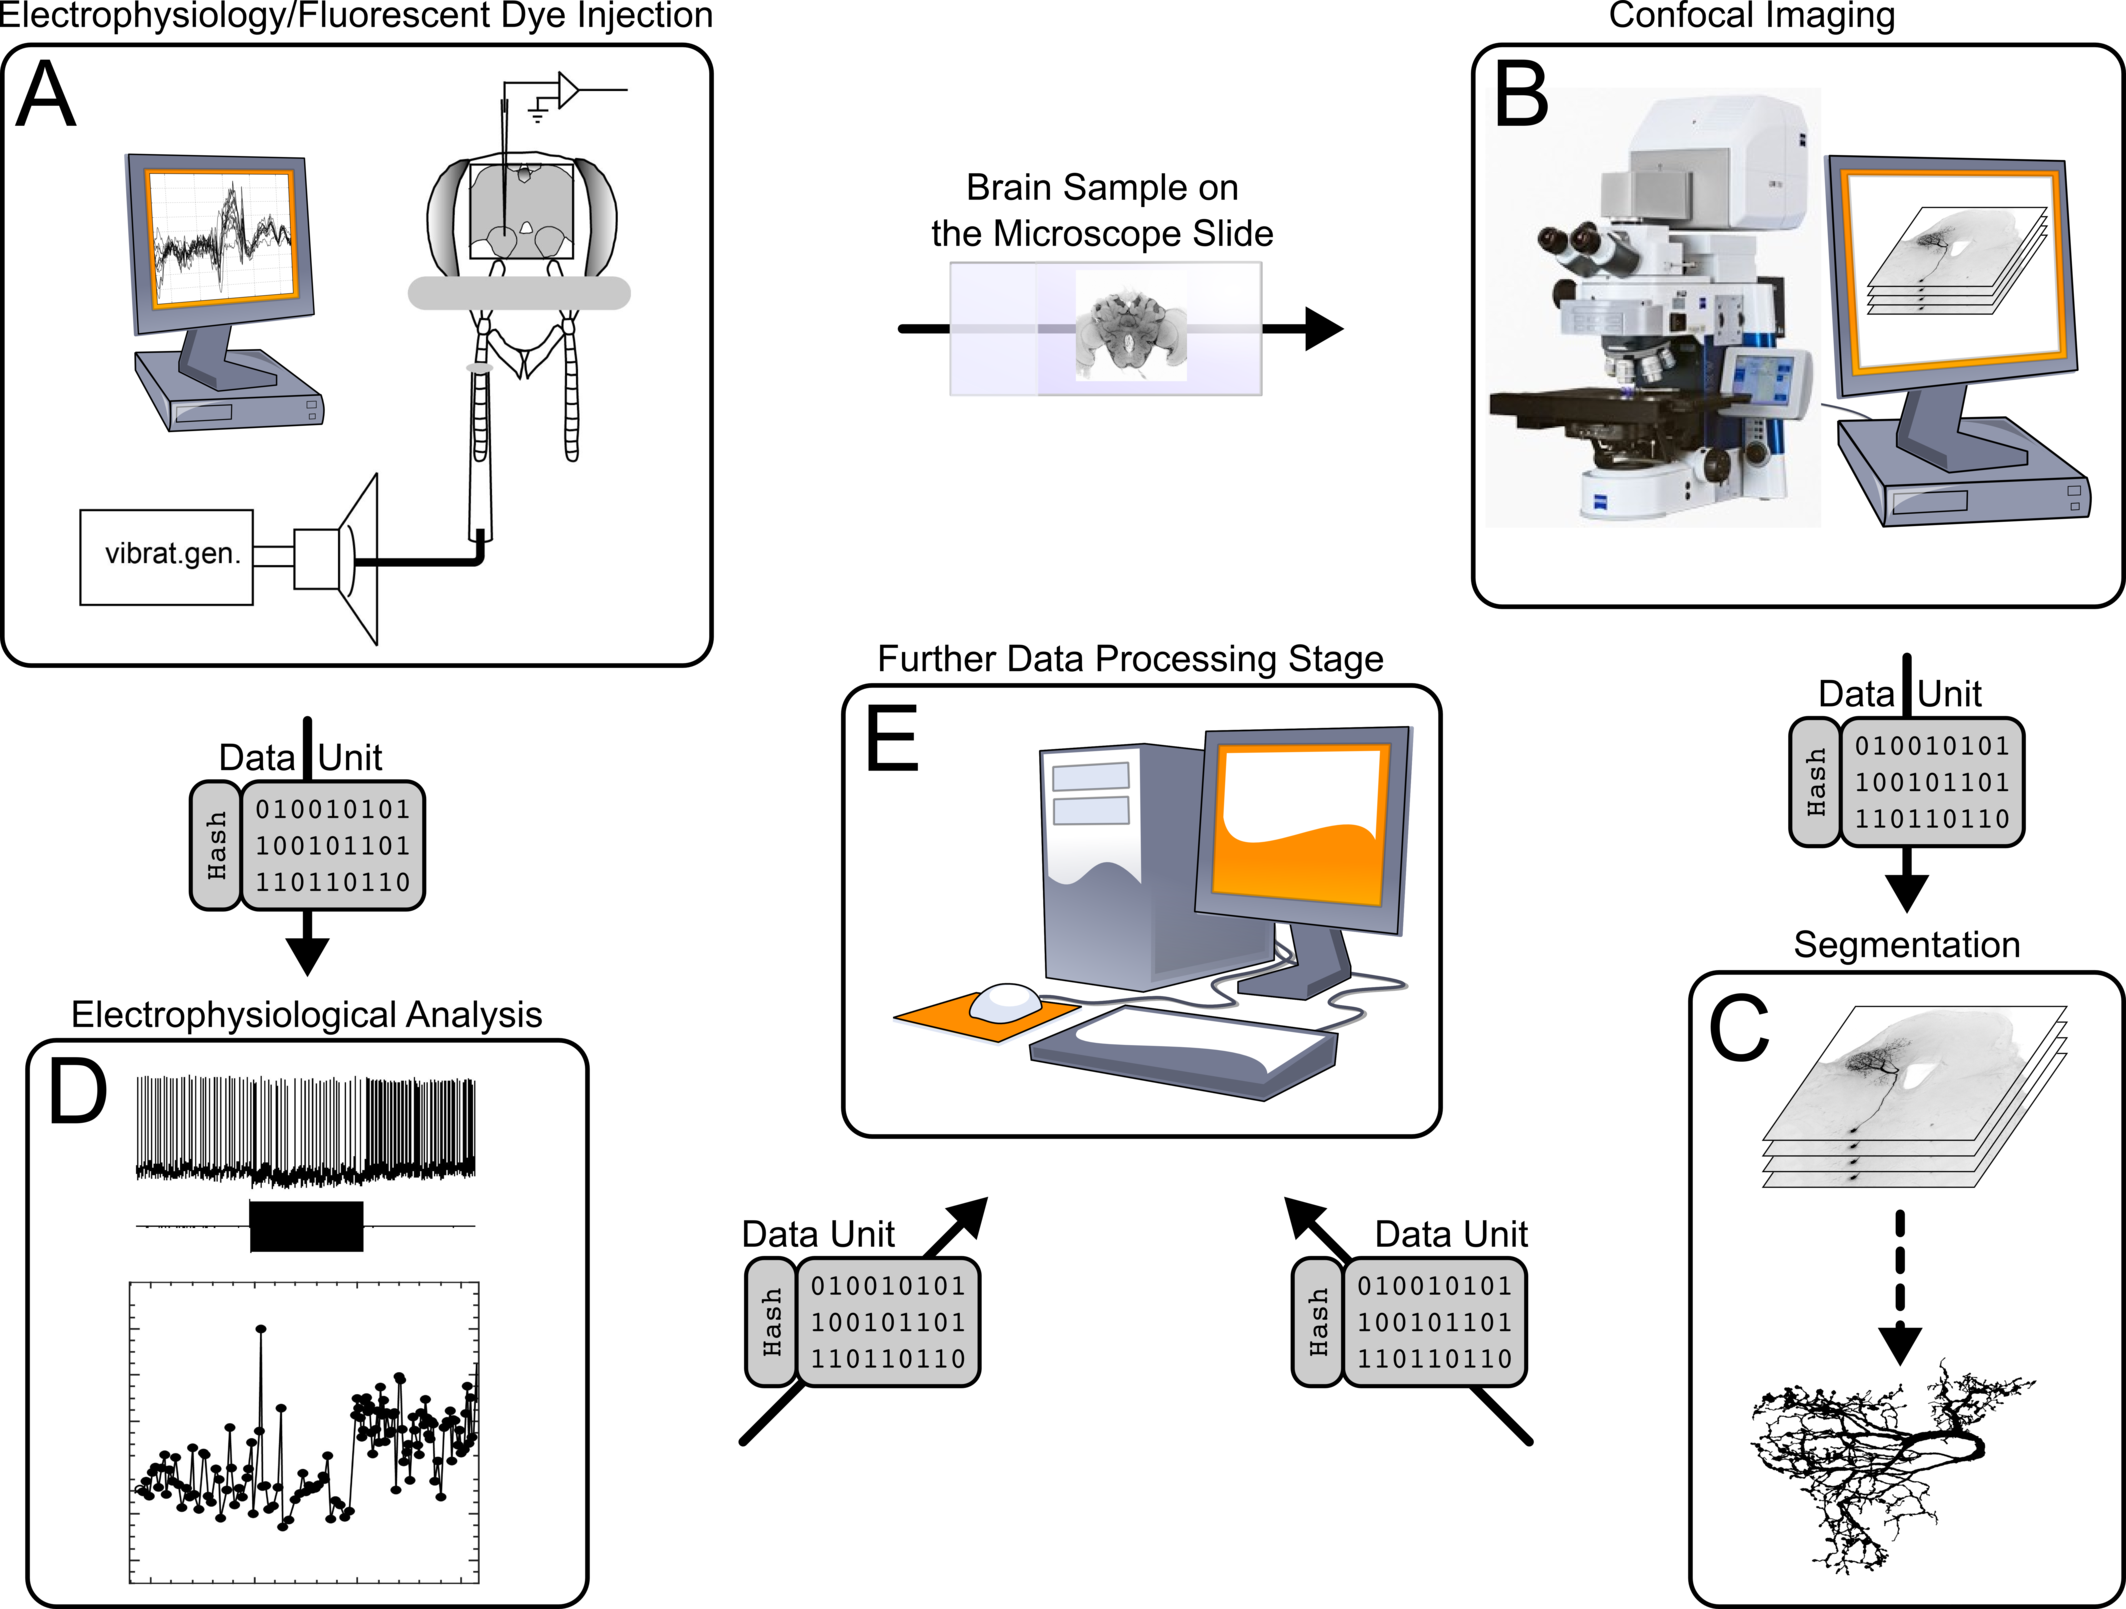
\includegraphics[width=\textwidth]{Figures/workflow}
\caption[Processing stages and data transitions]{
    \emph{Processing stages and data transitions of a typical workflow like the GinJang honeybee project}

    \textbf{I. Processing stages} (A) Single cell recording at a
    electrophysiological setup. Here, the electrical cell activity is measured
    at the dendrite, as well as a dye is injected into the cell. (B) Using the
    brain from experiments, image stacks are created applying confocal
    microscope technology. (C) The application SIGEN computes from confocal
    image stacks segmentations representing the underlying neuron. (D)
    Electrophysiological recordings are analyzed with specialized software.
    This stage represents an entire electrophysiological infrastructure using
    local computers at the experimental lab but also remote G-Node-services.
    For simplicity, this illustration exemplary shows the result of a spike
    detection algorithm identifies spikes of three neuronal units. (E) Further
    process stages follow building upon already processed data.

    \textbf{II. Traditional data transition} (A $\rightarrow$ B) The honeybee
    brain is physically moved from electrophysiological setup to the confocal
    microscope setup. (B $\rightarrow$ C; C $\rightarrow$ E) data units (single
    file, or set of files that represents a logical unit like all files of an
    image stack) are transferred by common tools, like USB-sticks, external
    hard drives, Dropbox, or simply as emails attachment. The same tools are
    applied for (A $\rightarrow$ D; D $\rightarrow$ E) but moreover dedicated
    web techniques for the domain of electrophysiological provided by G-Node
    are applied.
}
\label{fig:workflow} 
\end{figure}
The GinJang project uses the honeybee brain as a model for establishing the
NeuronDepot. Honeybee communicates the direction and distance to food sources
with hive-mates by waggle dance \citep{Frisch1967}. The hive-mates detect and
process airborne vibration caused by the bee's wingbeat during the waggle
dance, which consists of vibration pulses with a highly specific temporal
pattern. We have already identified several critical interneurons for
processing the airborne vibration \citep{Ai2007, Ai2009, Ai2010, Ai2012,
Ai2013}, however the neural processing of these
vibration signals has rarely been studied, and the types and roles of the
neurons involved, their circuitry and its development are largely unknown. 

Members of the GinJang project also developed a program (SIGEN, see
\citep{Minemoto}) that automatically extracts and segments the morphology of the
critical interneurons in the vibration processing. GinJang project will clarify
the morphological characteristics of the vibration-processing neurons and their
morphological development of the neuron depending on the age and on the
experiences of dance communication.  

We describe next the workflow of an extract of the GinJang project, a
sophisticated use-case representative for NeuronDepot
(Fig.~\ref{fig:workflow},~\ref{fig:workflow_sequence}). The experimental setup
of the GinJang project is at Fukuoka University where electrophysiological
measurements (Fig.~\ref{fig:workflow}A), electrophysiological analyses
(Fig.~\ref{fig:workflow}D), and imaging (Fig.~\ref{fig:workflow}B) are
performed. The resulting image stacks are used at the University of Hyogo for
neuronal segmentation (Fig.~\ref{fig:workflow}C). These 3D neuronal segmentations are then
normalized by registering them into the Honeybee standard brain back at Fukuoka
University. Finally, morphological analyses, simulations, and further analyses
are done at Ludwig-Maximilians-Universität München (LMU) in Germany
(Fig.~\ref{fig:workflow}E).


\begin{figure}
\centering
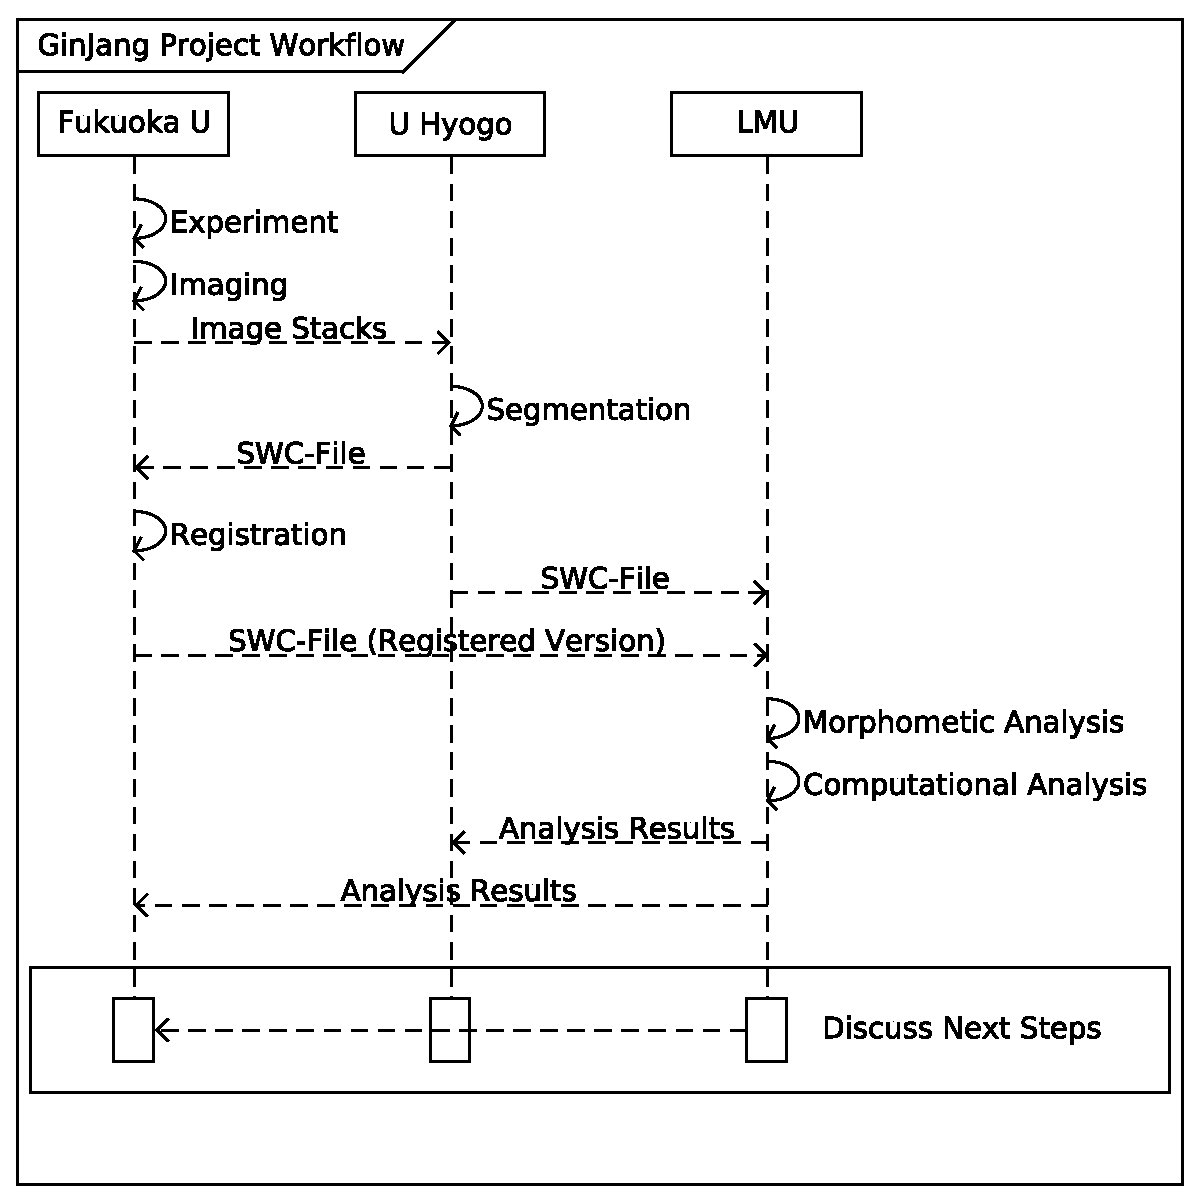
\includegraphics[width=8cm]{Figures/workflow_sequence.eps}
\caption[Sequence of GinJang Workflow]{
    \emph{Sequence Diagram of the GinJang workflow (morphological
    scope)}\pr{This figure will appear in one column within the final layout}

    The GinJang workflow starts at the Fukuoka University with two processing
    stages (indicated by solid arrows): the experimental data collection and the
    imaging processing stage. Anatomical image stacks are transferred (dashed
    arrow) to University of Hyogo where they are segmented. Segmented neurons
    are transferred to the LMU and also back to Fukuoka University where they
    are registered to the honeybee standard brain. Unregistered segmentation
    and registered segmentation are used for simulations and analysis at the
    LMU. Using analysis results, scientists in Fukuoka can tweak existing
    experiments or design new ones.
}
\label{fig:workflow_sequence}
\end{figure}


\subsubsection{Experiment}

The vibration-sensitive neurons in the honeybee auditory system
\citep{Ai2009}
are electrophysiologically and anatomically characterized at Fukuoka
University. Using sharp electrodes, voltage traces are recorded from
interneurons in response to several sensory input protocols \citep{Ai2009,
Ai2012, Kai2013}. Then the neuron is filled with a dye and
imaged at a different setup using confocal microscopy to generate anatomical
image stacks \citep{Ai2010, Ai2013}. Thus, every experiment generates
three kinds of data-metadata bundles:

\begin{itemize}
\item Electrophysiological data. E.g.: voltage and current traces
\item Microscopy image stacks
\item Honeybee metadata (e.g. age or colony) and neuron metadata (e.g. phenotype) Segmentation
\end{itemize}

\subsubsection{Segmentation}

Image stacks are transferred to the University of Hyogo, Japan. Here, using
automated image analysis software SIGEN \citep{Yamasaki2006, Minemoto} the 3D structure of the neuron is extracted and stored using the
SWC file format. At this stage two kinds of data are generated:

\begin{itemize}
\item Segmented neuron. E.g.: SWC file
\item Parameters used for segmentation (which constitute segmentation metadata)
\end{itemize}


\subsubsection{Registration}

The morphological segmentations of the neurons are transferred back to Fukuoka
University for registration into the Honeybee Standard Brain using various
transformations. We use the honeybee standard brain (HSB) to analyze the
spatial relationships among morphologically and physiologically characterized
vibration-sensitive neurons. The neuronal profiles of stained interneurons,
obtained from different preparations, are segmented  using Amira 4.1
\citep{Evers2005}. Subsequently, the neuropilar outlines are traced manually and
segmented with the Amira 4.1 label field editor. These neuropilar label fields
are used to register the segmented neuron of each preparation into the HSB
following the method described by \citet{Brandt2005}.


\subsubsection{Analysis}

These segmentations  (both registered and unregistered) are transferred to the
LMU, Germany where 3D segmentations are used for morphometric analysis and
simulation studies. Multiple kinds of data are generated at this
stage:

\begin{itemize}
\item model files for simulations
\item simulation metadata, e.g.: parameters of simulation, location of
    stimulation (input) and measurements (output)
\item simulation results: visualizations and summary data
\item morphometric analysis metadata, e.g.: subregion of analysis, metrics used
\item results of morphometric analysis: volume, surface area, number of branch points
\end{itemize}


\subsubsection{Traditional Data Transfer Methods}

The workflow of the GinJang project requires multiple data transfers between
diverse processing stages. These transfers were previously done via e-mail,
usb-sticks, external hard drives, ftp-servers, or cloud storage services (like
Dropbox, \url{http://www.dropbox.com/}). NeuronDepot replaces these traditional data transfer methods.


%%%%%%%%%%%%%%
% Requirements
%%%%%%%%%%%%%%

\section{Requirements}
We asked the members of the Ginjang Project to specify the features that they
expect to have in  NeuronDepot. Based on those we came up with the set of
following generalized requirements:
\begin{enumerate}
\item Data Management
    \begin{itemize}
    \item Replacement of "manual" data transitions using memory devices like
    e-mail, usb-sticks, external hard drives, ftp-servers, or cloud storage
    services
    \item Ease of metadata assignment for various kinds of data, like image stacks,
    voltage trace, neuronal reconstructions
    \item Visibility of  the current state of the project through a web browser
    \item Automatic update and synchronization across project workstations
    \end{itemize}
\item Integration
    \begin{itemize}
    \item Maintenance of the well established work environments of the participating scientists
    \item Minimization of the integration effort
    \end{itemize}
\item Data Security
    \begin{itemize}
    \item Reliability of upload and download of large data
    \item Access control
    \end{itemize}
\item Automated Backup
\item Additional Requirements
    \begin{itemize}
    \item Easy adaptation to new data-specific requirements that emerge during project
    \item Support for automated data-processing (cleaning, metadata extraction,
    analysis and simulation scripts)
    \item Quick overview of contents and metadata
    \item Flexible search of data
    \end{itemize}
\end{enumerate}


\begin{figure}
\centering
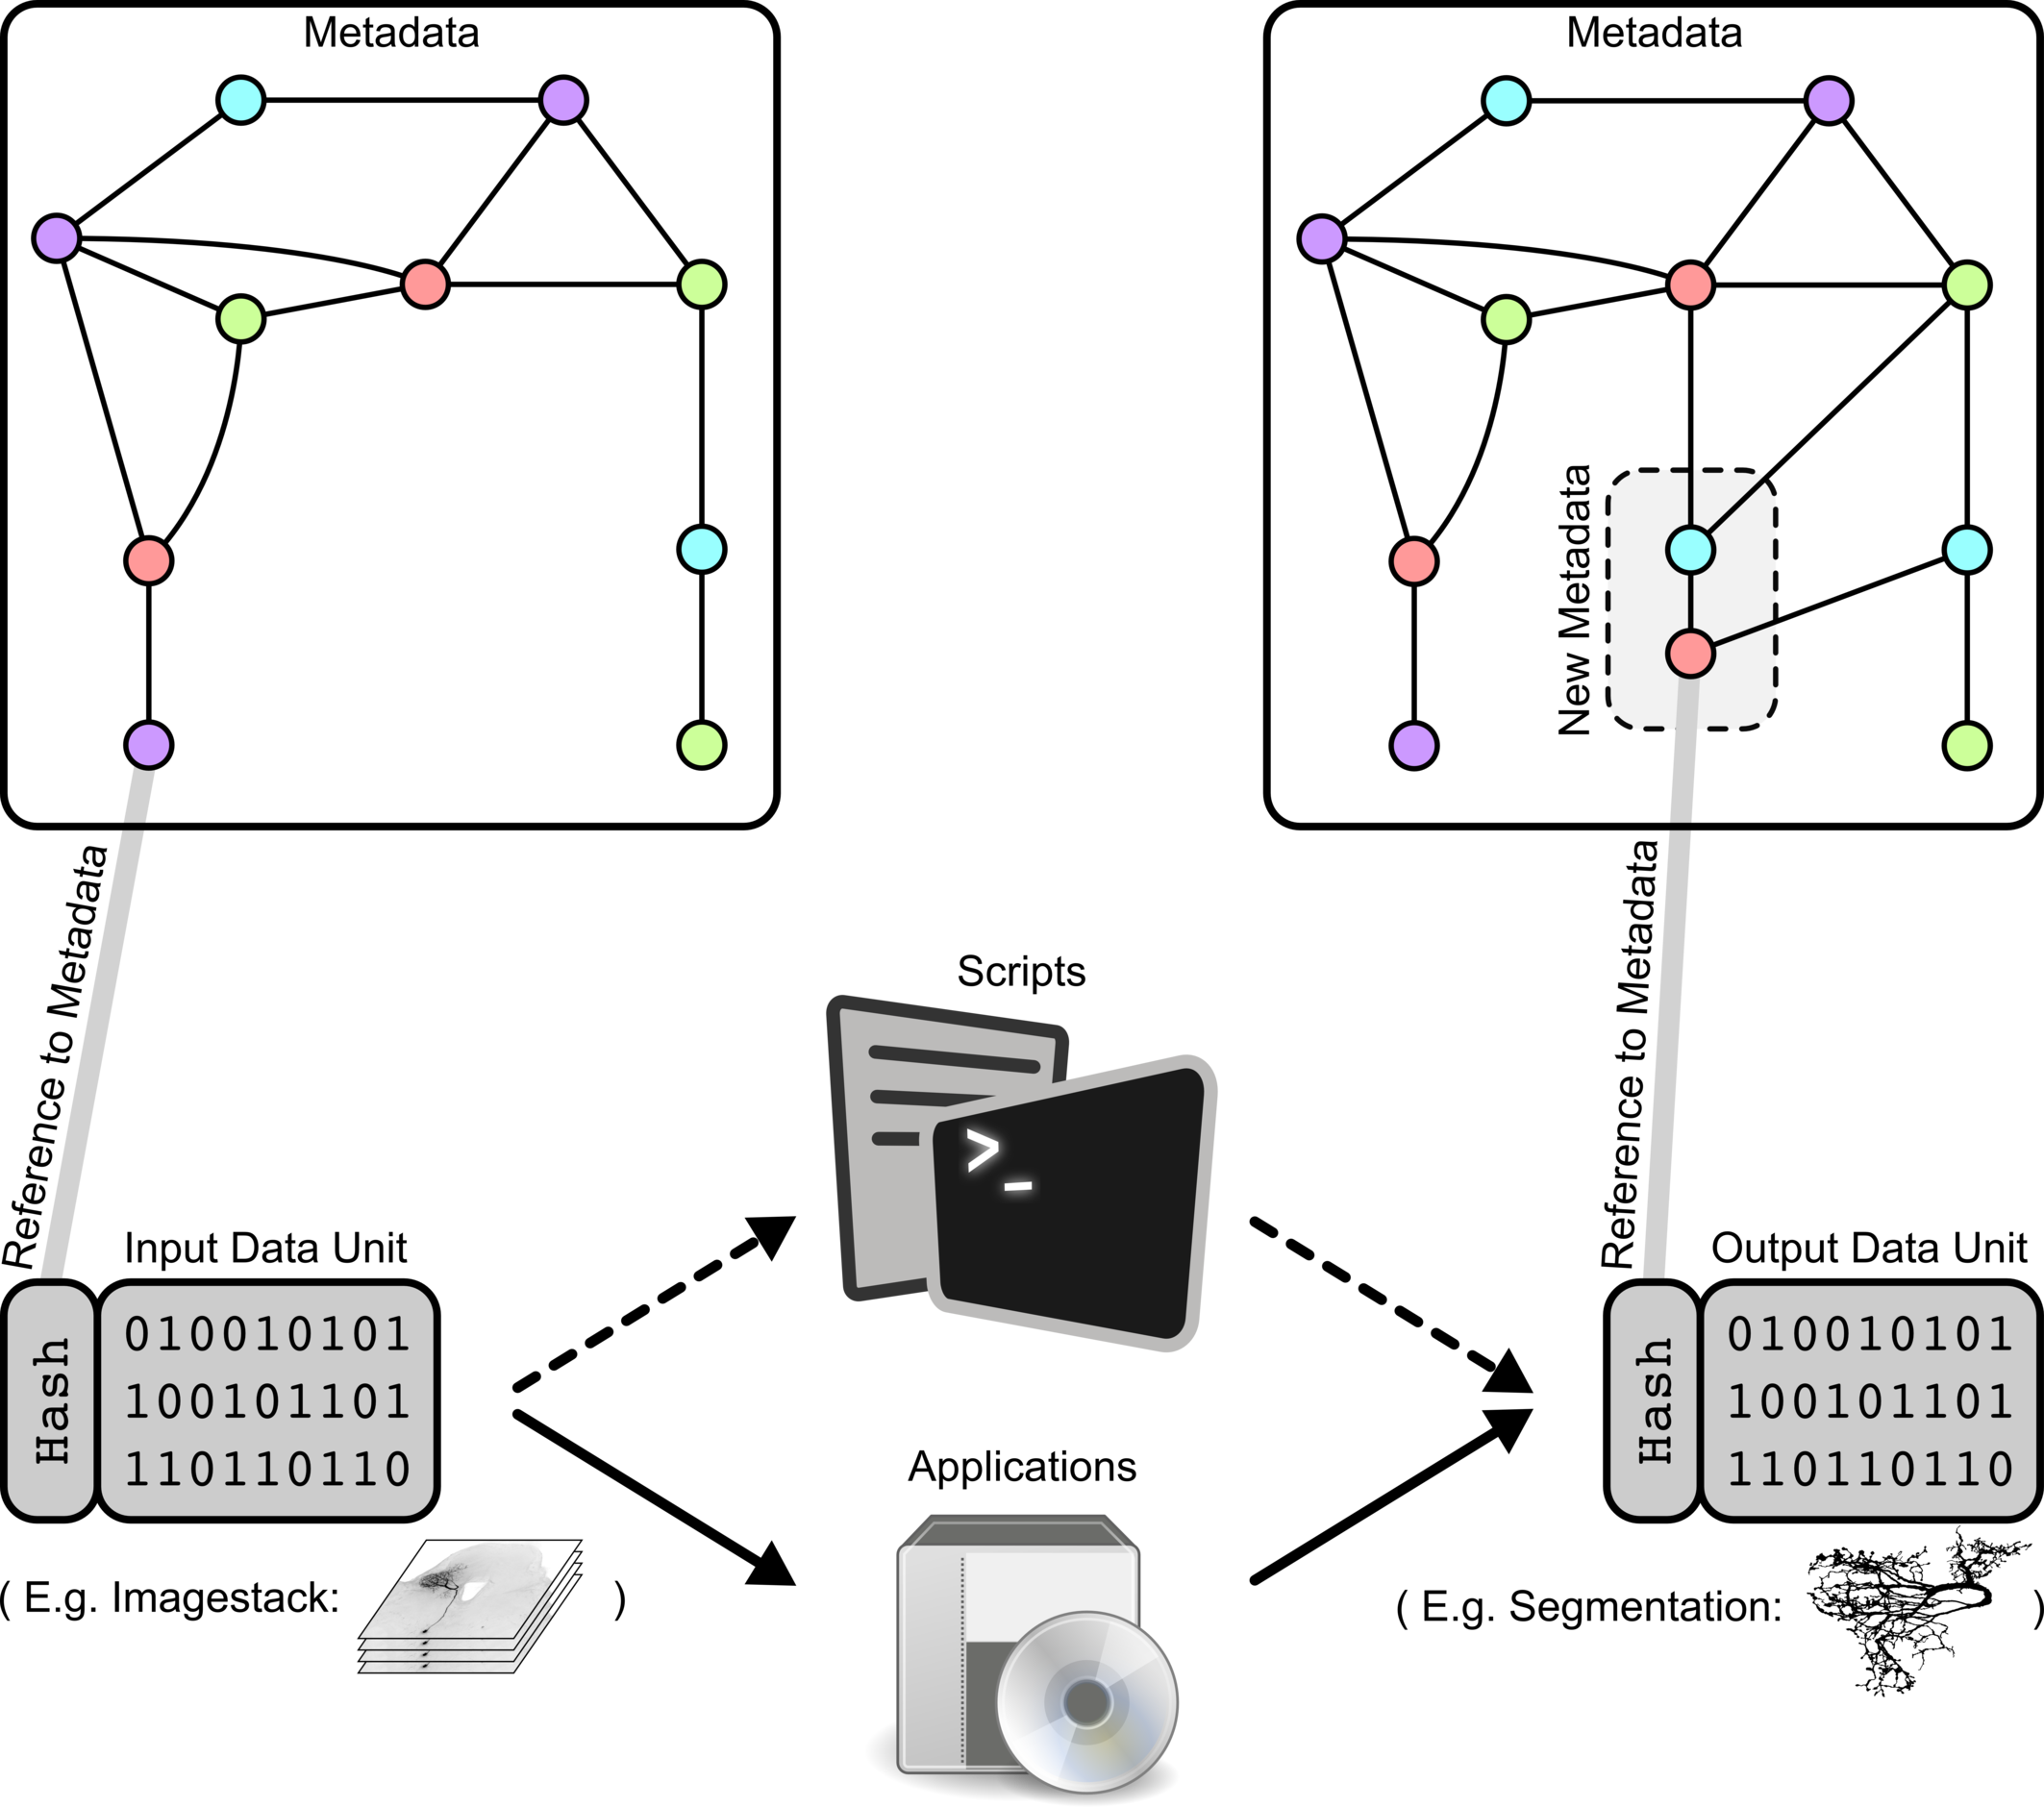
\includegraphics[width=\textwidth]{Figures/Metadata_DataUnits}
\caption[Metadata and Data Units]{
    \emph{Data units as smallest logical entity for specific data processing attached
    to the metadata of the project}

    (Left) A data unit is connected to metadata by its unique hash value id.
    Metadata is illustrated here as a graph where each points represents an
    attribute like \texttt{AGE=15}, \texttt{DATE=130525}, or
    \texttt{HONEYBEE=HB123}. The data unit could express an image stack, or a
    compartmental reconstruction of a specific neuron. (Middle) Data processing by
    a script or an applications that operates on specific input data units and that
    generates a new output data unit. For example, SIGEN generates from input data
    units expressing image stacks neural segmentations as an output data unit
    containing an SWC-file. (Right) Processing a data unit with a specific script
    or application leads to an output data unit associated with new metadata that
    is integrated into the existing metadata graph. According to our SIGEN-example,
    parameters of the segmentation algorithm are stored within the metadata graph.
}
\label{fig:metadata_dataunits} 
\end{figure}
%%%%%%%%%
% Concept
%%%%%%%%%

\section{Concept}

The key element behind NeuronDepot is a simple yet flexible schema for the data
that enables the construction of  hierarchical views. Such views are suitable
to be projected into filesystem trees. These projections can then be
synchronized via any cloud storage layer. 

The NeuronDepot approach is extremely simple. Assigning data units (see
definitions below) to a simple core schema enables to produce flexible
hierarchical views of the data in the form of context trees that provide a
context path for each data unit. Such hierarchical views gain interest because
they can be reshaped at will for specific processing needs, and are naturally
adapted for the use of filesystem tools, singularly cloud synchronization
software. Definitions for the emphasized terms are provided next.


\subsection{Definitions}

In the next parts, we will refere to the following definitions:

\textbf{Data unit:} A data unit (Fig.~\ref{fig:metadata_dataunits}, bottom
left and bottom right) is a logical grouping of one (trivial case) or multiple
files which are generated by a single process. This process can be an
experiment, an algorithmic data transformation or a simulation. Examples of
individual data units in the GinJang context include: an image stack consisting
of several image files, the morphology of a neuron represented in a single
SWC-file, or several plots and tables resulting from simulations of a neuron's
electrophysiological characteristics.

\textbf{Context Path and Context Trees:} Any data unit can be uniquely
identified by a subset of the metadata attributes associated with it
(Fig.~\ref{fig:metadata_dataunits}). We define the context path of a data unit
as an ordered list of the specific attributes that uniquely identify it
(Fig.~\ref{fig:context_tree}). This context path can be used to construct a
path in the file system where the order of metadata attributes corresponds to
the hierarchical levels in the file system. 

\begin{figure}
\centering
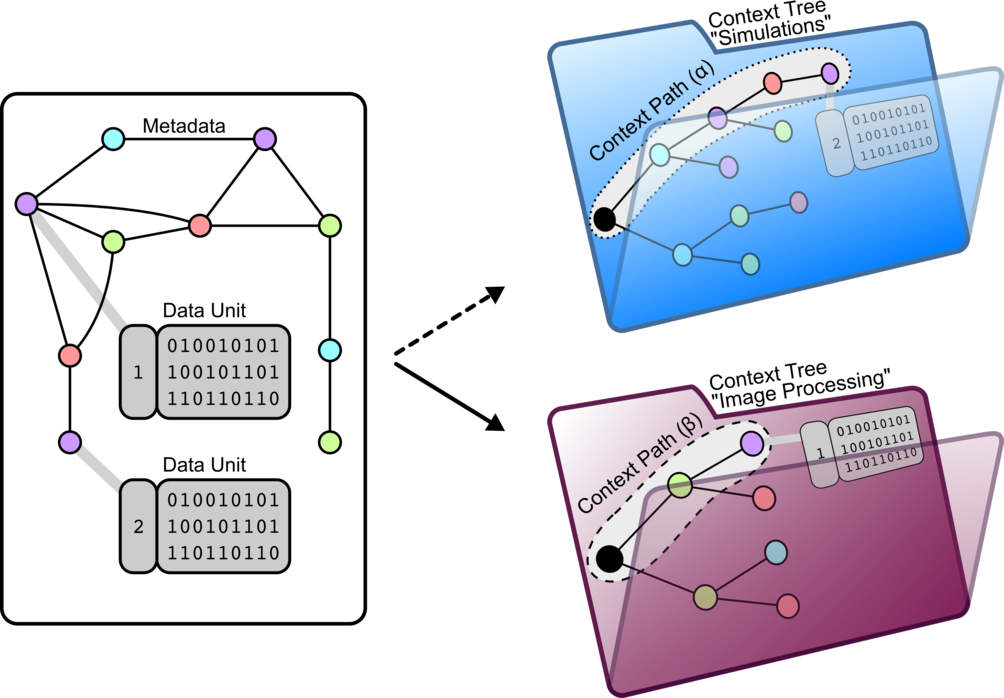
\includegraphics[width=85mm]{Figures/ContextTree}
\caption[Mapping data units to context trees]{
    \emph{Mapping a data unit to Context Trees using attached metadata}
    \pr{This figure will appear in one column within the final layout}

    (Left) Each data unit is connected to metadata. Using this metadata allows
    the organization of data units by two aspects: The entire data of a project
    can be (1) sub-divided into divers subsets of data where (2) data units are
    arranged within a tree structure where the nodes represent metadata and the
    leafs represent the data unit. As a meaningful specification of such a
    arrangement depends on the context of data usage, we call this arrangement
    \emph{Context Tree}.
    (Right) One Context Tree of NeuronDepot arranges project
    data for our morphometric processing stage. The file format \texttt{SWC} serves as
    a filter argument as just SWC-files are needed for simulation. Metadata
    attributes \texttt{LABOR\_STATE}, \texttt{REGION}, \texttt{HONEYBEE\_ID}, and
    \texttt{SIGEN\_PARAMETERS}
    serve for grouping.
    
    \emph{Example of Context Path ($\alpha$) pointing to a data unit containing a
    segmentation:}
    \texttt{/forager/left\_DL/HB130427/D20V05C01S01/morphology.swc} Another
    Context Tree of NeuronDepot arranges project data for our imaging
    processing stage.  Here, the project data is reduced to image stacks.
    Metadata attributes \texttt{HONEYBEE\_ID} and \texttt{REGION} serve for
    grouping.

    \emph{Example of Context Path ($\beta$) pointing to the same data unit:} \texttt{/HB130427/left-DL/*.tiff}
}
\label{fig:context_tree} 
\end{figure}

\emph{Example}: If a member of the project wants to analyze one particular
segmentation-data unit of neuron \texttt{NRN-1} of honeybee \texttt{HB123}, the following two
paths would represent these attributes:

\begin{lstlisting}[style=display]
(1) HB123/NRN-1/segmentation/
(2) segmentation/HB123/NRN-1/
\end{lstlisting}


The ideal order of the attributes depends on how the data units are to be
queried for specific analyses: the path order is projected into a hierarchy and
therefore defines different grouping levels specific analyses.

\subsection{Core Ideas}
\subsubsection{Hierarchical Arrangement of Data}

NeuronDepot applies systematically the principle of using of folder and file
names as metadata for the data contained in the filesystem. For flexibility,
the collection of data units is stored in a central server in a flat structure
where each data unit has a unique identifier, and the metadata is kept separate
and referenced to those identifiers. When a user defines the subset of data she
is interested in, along with a hierarchical arrangement that suits her needs
(what we call a projection) NeuronDepot creates a user- and task-specific
context tree as a hierarchy of symbolic links with the data units sitting at
the leaves. By exposing these hierarchies to a synchronization daemon, the
projection is made available to every workstation that subscribes to it.

NeuronDepot also leverages the advances in synchronization technology for the
data upload process: the user simply places new data units in a designated
floating folder (i.e. a folder outside the context tree). This folder is
synchronized to the server. The data units appear then as available for
metadata assignment via the NeuronDepot web app. Once metadata assignment is
complete, data units can be projected, as described above, to hierarchies that
are adapted to the local users' workflows. Data units are now also accessible
to cloud analytic services that directly query the metadata database without
demanding a specific projection, as these clients are not constrained by the
hierarchical data model of filesystems. NeuronDepot thus maintains consistency
all the way from the scientists' local copy of acquired data to the cloud-based
analysis platforms.


\subsubsection{Cloud-Based Data Flow}

NeuronDepot's mechanism for data transmission is based on synchronization by
cloud storage services (Fig.~\ref{fig:cloud_concept}). Cloud storage services
are used to keep all local computers that are involved in the project updated
by the server and, therefore, updated among each other. This core update
process is based on synchronization on the file system level. In order to
integrate data units into workflows, the system provides two types of base
folders: floating folders (Fig.~\ref{fig:cloud_concept}-1) and context tree
folders(Fig.~\ref{fig:cloud_concept}-3). Floating folders are provided with
read/write permissions for project members (we call it floating folder, as data
within that folder is not assigned to the metadata structure and therefore in a
floating state ). Floating folders are part of the data-assignment process
(Fig.~\ref{fig:cloud_concept}-2) . The second type of folder is the context
tree folder with read-only permissions for project members that synchronize
projected context trees to the local work environment.

\begin{figure}
\centering
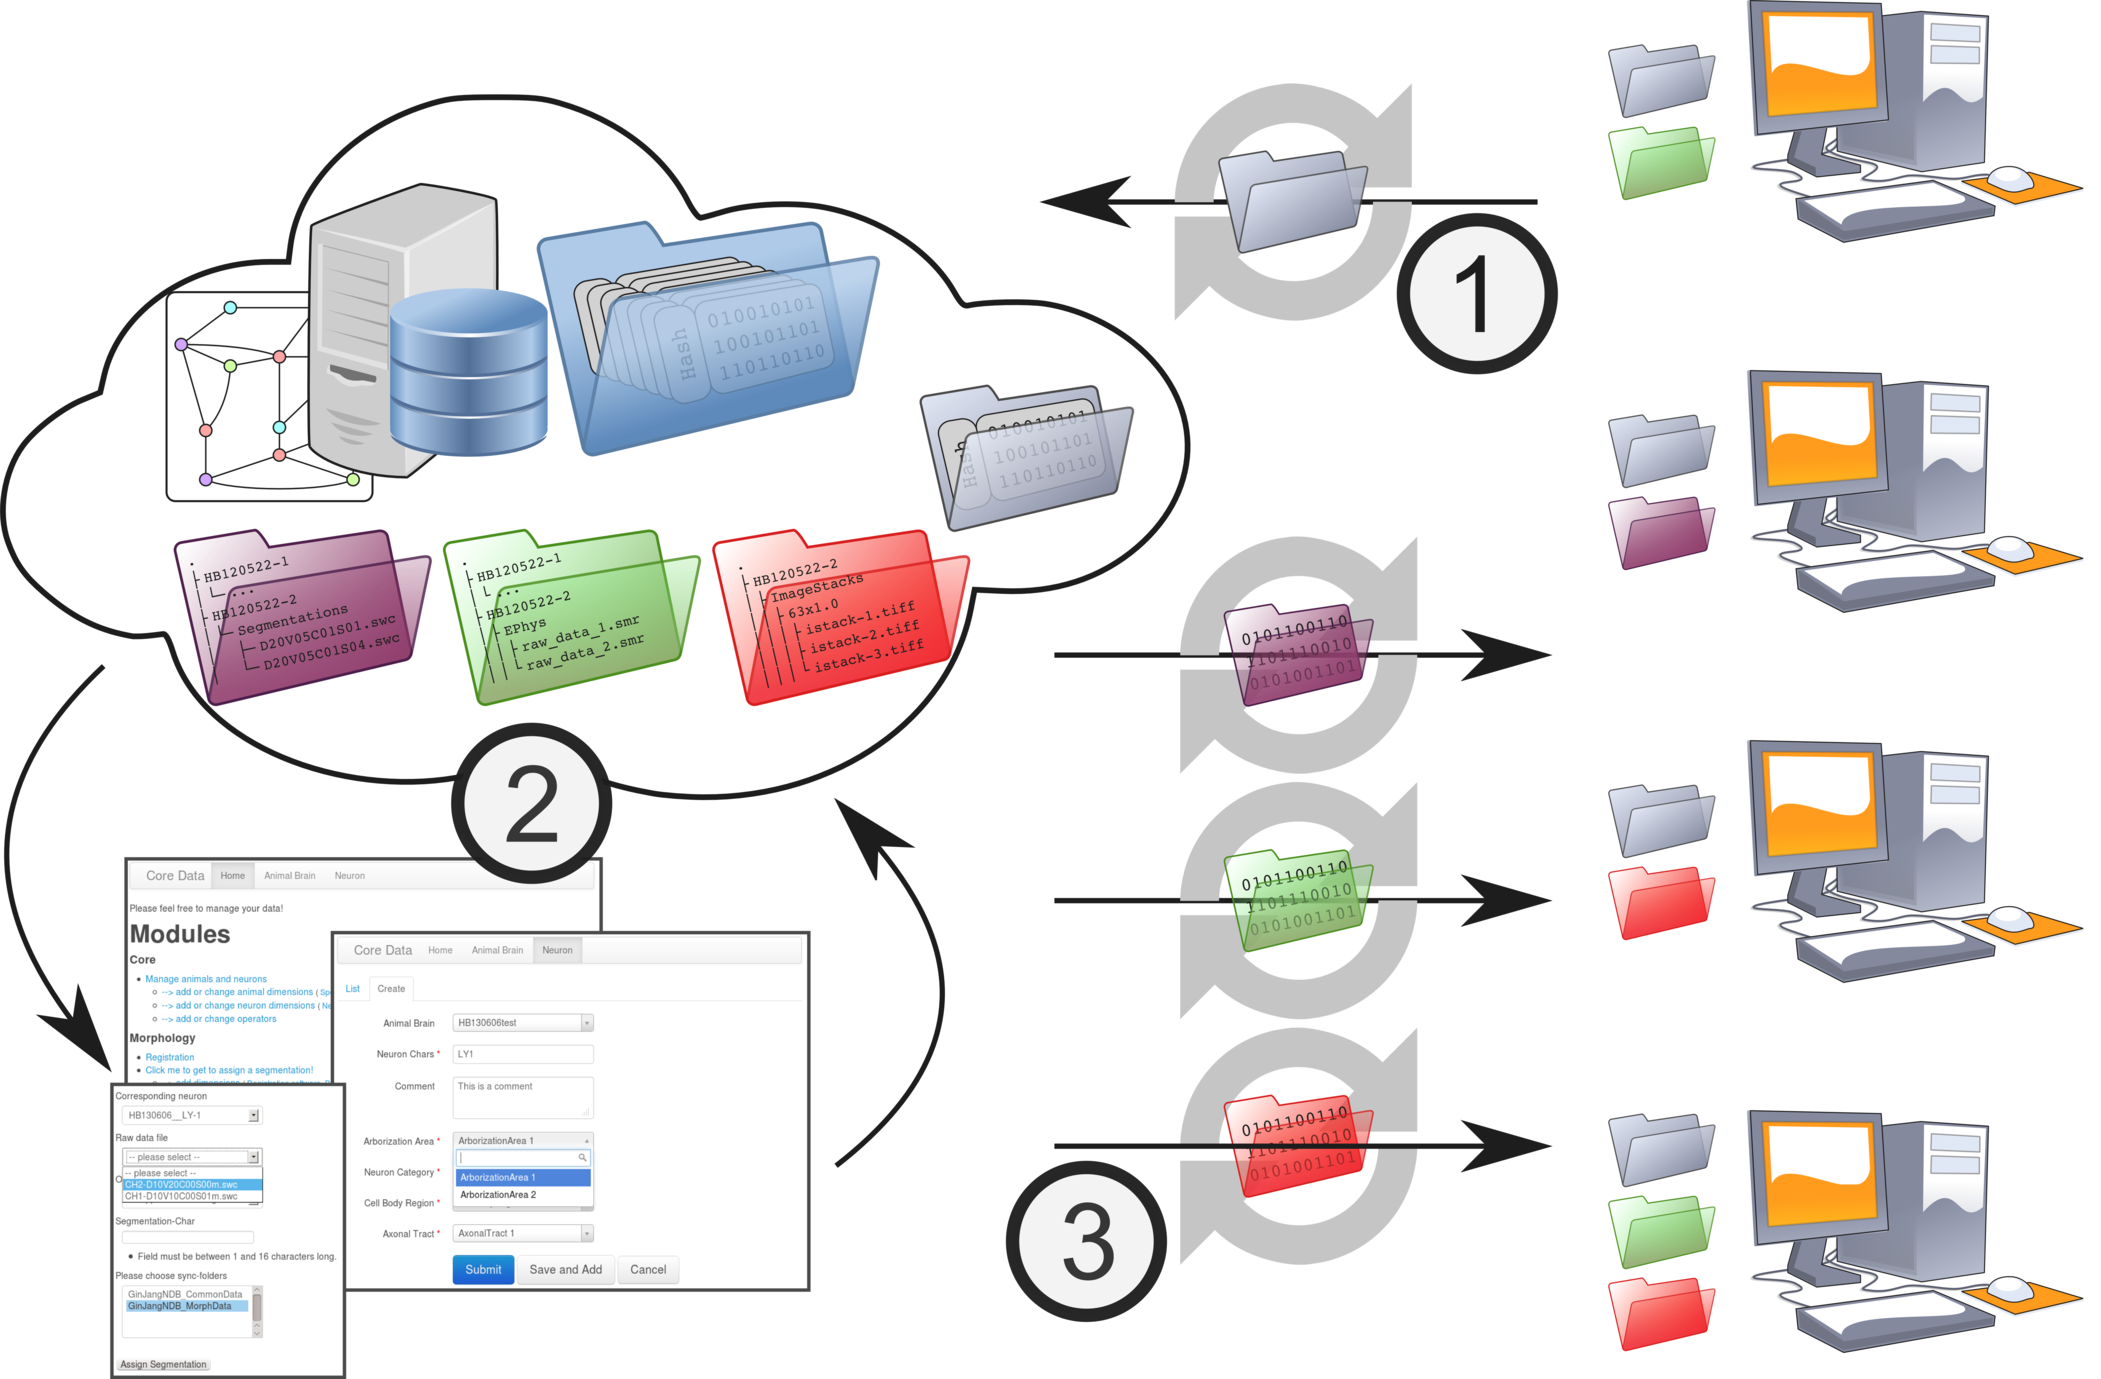
\includegraphics[width=\textwidth]{Figures/cloud_concept}
\caption[Schematic depicting NeuronDepot]{
    \emph{Schematic depicting NeuronDepot's data flow}

    NeuronDepot is based on cloud storage services and user-friendly web-app
    services that use modern database management systems. Cloud storage
    services are used to keep all local computers that are involved in the
    project synchronized with the server and, therefore, synchronized among
    each other.  This core synchronization is based on the file system. In
    order to integrate files into our workflows, our system provides two types
    of base folders: floating folders for upload (gray, here just one) with
    read/write permissions for project members and multiple data folders
    (purple, green, red) with read-only permissions for project members.

    The new data transition workflow consists of three steps: (1) new data
    units are stored at the floating folder and synchronized to the server in
    the background. (2) Synchronized data units are assigned to the existing
    project data via a web application (as NeuronDepot's web-application uses
    responsive features, it can be used from divers devices like smart phones,
    tablet PCs, or traditional desktop computers). The system assures that all
    data is correctly related to each other and that all data stays consistent.
    Project members can plug scripts into this assignment process to automate
    and facilitate data processing. Moreover, the system provides divers
    reports to brief the scientists about the current state, or about recent
    changes. (3) NeuronDepot distributes data units back to project members.
    According to the underlying context tree, NeuronDepot projects the folders
    synchronized by cloud storage services.
}
\label{fig:cloud_concept} 
\end{figure}

The underlying data transfer workflow replaces traditional transfer methods as
described above by these folders which are organized by consists of three
steps: (1) new data units are stored within the floating folder and
synchronized to the server. (2) Synchronized data units within the floating
folder are assigned to the existing project data via a web application. As
NeuronDepot's web GUI uses responsive features, data can be assigned from
diverse devices like smart phones, tablet PCs, or traditional desktop
computers. The system assures that all data is correctly related to each other
and that all data stays consistent. Project members can plug scripts into this
assignment process to automate and facilitate data processing. Moreover, the
system provides diverse reports to brief the scientists about the current
state, or about recent changes. (3) NeuronDepot distributes data units back to
project members. According to the underlying context tree, NeuronDepot
synchronizes projected context tree folders by cloud storage services to the
workstations of the scientists.

%%%%%%%%%%%%%%%%%%%%%%%
% Design Considerations
%%%%%%%%%%%%%%%%%%%%%%%

\section{Design Considerations}
The architecture of NeuronDeport follows these principles:

\textbf{Incorporation of existing open source components} \texttt{  } The open source ecosystem holds multiple solutions solving very specific tasks.
E.g. controlling the persistence of objects by mapping them to database
structures, solving numerical tasks highly optimized, or illustrate data by
drawing graphs and figures. Moreover, the community of neuroinformatics have
added  very domain specific tools for simulations, analysis, and processing of
data from the field.

\textbf{Utalization of established cloud services} \texttt{  } Over the past
few years, cloud computing has rapidly emerged as a widely accepted computing
paradigm built around core concepts such as on-demand computing resources,
elastic scaling, elimination of up-front investment, reduction of operational
expenses, and establishing a pay-per-use business model for information
technology and computing services. There are different models of cloud
computing that are offered today as service, such as software as a service
(SaaS), platform as a service (PaaS), and infrastructure as a service (IaaS)
\citep{Mell2011, Azodolmolky2013}. The use of cloud computing services helps to
reduce the development time and effort.

%%%%%%%%%%%%%%%%%%%%%
% System Architecture
%%%%%%%%%%%%%%%%%%%%%
\section{System Architecture}

\begin{figure}
\centering
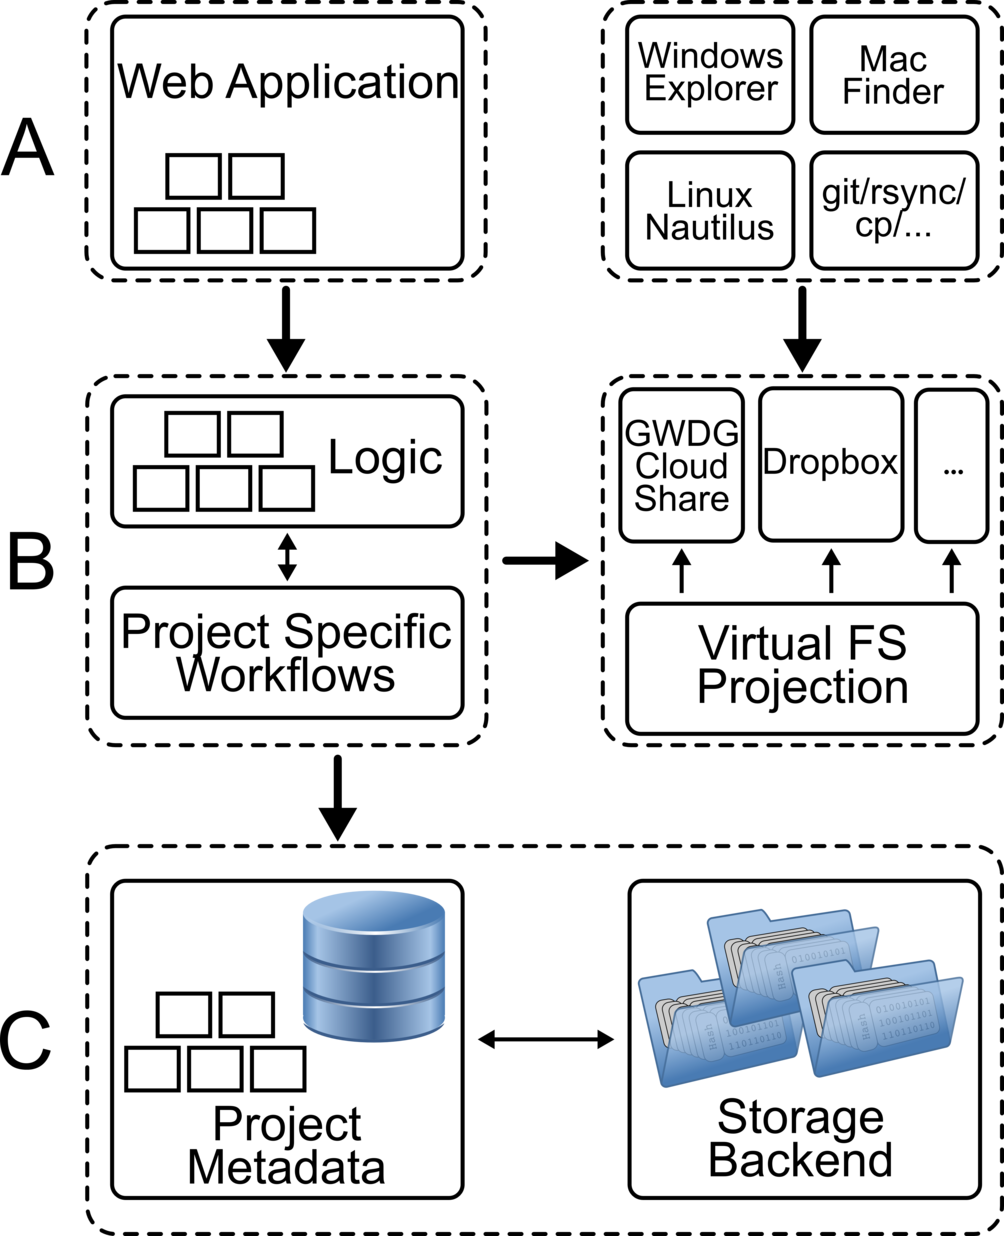
\includegraphics[width=85mm]{Figures/architecture}
\caption[System Architecture]{
    \emph{System architecture}
    \pr{This figure will appear in one column within the final layout}
    
    (A) The graphical user interface  consists of two parts: a web application
    and local applications. The web application (\emph{left}) provides forms
    for assigning data, enter metadata, and annotating data with metadata. The
    upload and download processes are handled by cloud services incorporated by
    our filesystem projection layer (see below). Here, scientists can use
    established tools like Windows Explorer, Mac Finder, Linux Nautilus, or
    other file managers to copy files for upload in dedicated folders
    (\emph{right}) which are connected to the cloud services.
    (B) The business logic (\emph{left}) encodes the NeuronDepot logic rules
    that determin how data can be created, red, updated, and deleted.
    Moreover, when new data items are added, deleted or modified, project
    specific workflows can be triggered. The workflows are purely computational
    and are composed of multiple tasks and can be specified for each processing
    stage (\emph{small rectangle}). Because the workflows are executed
    asynchronously, a consistent view of the storage backend is needed. A
    Virtual Filesystem Projection layer (right) maps data items and directories
    to cloud storage synchronization clients based on project specific metadata
    and provides a consistent view of the file system structure for
    computational workflows.
    (C) Within a project database additional metadata is stored. This can be
    metadata which was extracted by a computational workflow or manually
    entered data. The responsibility of the storage backend is to consistently
    store data items and provide abstractions for the file system projection
    layer.
}
\label{fig:architecture} 
\end{figure}

\subsection{Graphical User Interface}
The architecture underlying NeuronDepot consists of individual layers (Fig. 6). Users can access NeuronDepot via a web application or through cloud storage synchronization clients.

The graphical user interface (GUI) consists of two parts: a web application
(Fig.~\ref{fig:architecture}A, left) and local applications
(Fig.~\ref{fig:architecture}, right). The web application provides forms for
assigning data, enter metadata, and annotating data with metadata. We used
the micro web framework Python-Flask (\url{http://flask.pocoo.org/}) for rapid
development.

The upload and download processes are handled by cloud services incorporated by
our filesystem projection layer (see below). Here, scientists can use
established tools like Windows Explorer, Mac Finder, Linux Nautilus, or other
file managers to copy files for upload in dedicated folders
(Fig.~\ref{fig:architecture}A, right).  Clients like Dropbox, Google Drive
(\url{https://drive.google.com/}), or GWDG Cloud Share
(\url{https://powerfolder.gwdg.de/}) are connected to the virtual filesystem
projection layer. 


\subsection{Business Logic and Virtual Filesystem Projection}\label{sec:projection_layer}

The business logic (Fig.~\ref{fig:architecture}B, left) encodes the NeuronDepot
logic rules that determin how data can be created, red, updated, and deleted.
Moreover, when new data items are added, deleted or modified, project specific
workflows can be triggered.  The workflows are purely computational and are
composed of multiple tasks. Because the workflows are executed asynchronously,
a consistent view of the storage backend is needed. We therefore propose a
Virtual Filesystem Projection layer (Fig.~\ref{fig:architecture}B, right) which
can map data items and directories to cloud storage synchronization clients
based on project specific metadata and provides a consistent view of the file
system structure for computational workflows.

The control-flow of a workflow is constructed out of multiple tasks. Typically
tasks extract metadata, index data items, manipulate images or calculate
statistics. Workflows are typically created in Python with the help of
libraries like Snakemake \citep{Koester2012}. Workflows in NeuronDepot should run
without specific adaptations.

Workflows can be triggered explicitly by user interactions over the web
frontend or implicitly by the Virtual Filesystem Projection layer when new
files are added. The execution state of the workflow is displayed in the web
application. The synchronization of the files between the researchers is done
asynchronously in the background with cloud synchronization clients, see (Fig.
6). Hence the execution of computational workflows  has to be deterministic
despite of asynchronous changes of files. This requirement is fulfilled by
persistent data structures (see ~\ref{sec:projection_layer}).

The filesystem projection layer projects the data items based on metadata to
directories and files. The hierarchy is stored in project metadata storage, the
data items in the storage backend.

A way to achieve this requirement is to serialize all changes at the server and
introduce persistent data structures~\cite{Driscoll1989}. The persistent data
structure is shared between the server and the computational workflow. One way
to share the data structure would be to implement a custom library for file
system access based on FUSE. Hence the workflow has a consistent view on the
data items until it finishes. When the workflow is finished, the changes are
committed. Given there was another modification while the workflow was running,
the transaction wouldn’t be able to commit. In this case the workflow could be
rerun based on the latest snapshot, or a new branch would be created. A
conceptual similar approach is transactional memory. Transactional memory
provides programming abstractions which makes it easier to develop
multithreaded applications (\url{http://clojure.org/refs}). In NeuronDepot we
want to use a similar approach to provide a consistent view on the data items
while a workflow is executed. The storage backend uses a SHA-1 hash as unique
identifier for the data item in the project bucket. Calculating a SHA-1 hash of
11.5GB file on a commodity laptop with a SSD took only about 41 seconds, hence
it is feasible to take a SHA-1 hash as the unique identifier.

This approach has also other advantages: The filesystem can be viewed to an
arbitrary point in time in the history of the project and no snapshots are
needed. This is also space efficient since it benefits from structural sharing
and doesn't have to keep snapshots of data items. The integrity of a file can
be checked by calculating the hash and comparing it.

\subsection{Persistence Layer}

The persistence layer (Fig.~\ref{fig:architecture}C) consists of the following two components:

\textbf{Project Metadata} \texttt{  } Within a project database additional
metadata is stored. This can be metadata which was extracted by a computational
workflow or manually entered data. For mapping Python objects to database
objects we use SQLAlchemy (\url{http://www.sqlalchemy.org/}) storing metadata
in an PostgreSQL (\url{http://www.postgresql.org/}).

\textbf{Storage Backend} \texttt{  } The responsibility of the storage backend
is to consistently store data items and provide abstractions for the file
system projection layer. The abstractions provided are similar to a key value
store. The Amazon S3 API distinguishes between buckets and objects
(\url{http://aws.amazon.com/documentation/s3/}). Objects, which are data items,
are put into buckets. Each bucket has a flat namespace. There are multiple open
source alternative implementations like RiakCS
(\url{https://github.com/basho/riak\_cs}) or OpenStack Storage
(\url{http://www.openstack.org/software/openstack-storage/}). For the storage
backend of NeuronDepot we are using a backend with a similar API. The hierarchy
of the backend filesystem is stored within the project specific metadata and
linked through a key. A key is created based on the SHA-1 hash of the data item
itself. With that the content of the file can be further checked for
corruptions.

\section{Discussion}

\subsection{Adaptability}
The system architecture of NeuronDepot can be conceptually divided into two
parts: the core engine which is not specific to any processing stage, and thin
modules which are project specific, e.g.: In the Ginjang project, segmentation
is a processing stage. A thin module provides all the required features for the
data and metadata produced by this processing stage like connecting it to other
existing data in NeuronDepot, handling upload of this data and specifying the
information necessary while presenting it to the user.

NeuronDepot can be adapted to other projects by incorporating project specific
thin modules upon its core engine. These thin modules correspond to the
different processing stages of a project, while the core engine
remains the same.

\subsection{Advantages over other existing systems}

Provision of data via a file system opens up plethora of tools that are
available at the local work bench, like (i) Desktop-Search using diverse
indexing methods (spotlight, locate, Copernic, Google-Desktop search) (ii) File
system explorers(for  searching and sorting) (iii) Backup (iv) Version-Control
(v) Unix-world applications like \texttt{grep, find, and tree} (since
"everything is a file") (vi) Transmission protocols like \texttt{ftp, ssh, and
http} (vii) File Synchronization Services.

Unlike with other existing solutions, using NeuronDepot does not require
learning a new GUI or any other infrastructure specific usage features since at
the user end, the data is provided as  a filesystem.

An important feature of NeuronDepot is the isolation of the upload process from
the GUI. Data is not uploaded by the user manually but is just assigned. The
user does not need to wait for the file to be uploaded.

At the end user, a subset of the data in the database is presented in a tree
structure. Here, what subset has to be presented and in what structure is
specified by the user. Such a representation of a desired subset of the data in
a hierarchical structure provides a partitioning/grouping of the data which
becomes very handy if the user intends to perform analysis or comparison on a
specific subset of the data.

As mentioned before, the upload process of NeuronDepot consists of two steps.
Data is copied into the virtual file system and then assigned from there to the
database using the GUI. This upload procedure facilitates assisted assignment
of data since the data is available beforehand. Certain analysis scripts can be
started on the data in the virtual file system and its results can be later
used during the assignment of the data via the web-GUI.

In NeuronDepot, a specific subset of data is encapsulated into an entity via
the concept of Context Trees. Such an encapsulation facilitates management
operations such as referencing, tagging and sharing, in which treatment of the
subset of the data as an entity is essential. This is very much like a book
encapsulating a set of concepts/facts and making them a single entity.

\subsection{Further Directions, Limitations, and Open Questions}

A package/extension for an existing web-framework like Flask or Django can be
developed by reorganizing the system components of NeuronDepot.  Several
existing solutions of the Open Source Ecosystem were used in the development of
NeuronDepot and this will be a way of contributing back to it.  Moreover, it
will serve as a good building block for the development of new data software.

Databases which
would support this kind of scenario would be MongoDB
(\url{http://www.mongodb.org/}) or CouchDB (\url{http://couchdb.apache.org/}).

Furthermore, adaptation of NeuronDepot for a specific project workflow is not
just a reconfiguration of the infrastructure. It also involves additional
scripting of thin modules. In the first step NeuronDepot will support only a
single core-engine with a single project. Support for multi tenancy
requires elaborate user and rights management which is planned in future. In
the first step this can be worked around by installing multiple instances.

At the moment, the context trees used to provide the user with data are hard
coded. The user has to communicate with the developers to have different data
structures provided to him. This process can be slow and can prove to be a
hindrance to the scientist's work. A service can be incorporated which enables
the user to specify what data structure he needs. This would reduce the user's
dependence on the developers and also allow the user to quickly adjust the data
that he requires from NeuronDepot.

\section{Conclusion}
With this software architecture, we contribute an approach to scientific data
worfklow and a tool to the ecosystem of neuroscientific software.  NeuronDepots
principal merit is to integrate smoothly with established tools and resolve the
transition from local to cloud-based processing, without requiring researchers
to relinquish control of their data or analysis but enabling them to leverage
the advantages of cloud services.

\section*{Disclosure/Conflict-of-Interest Statement}
%Frontiers follows the recommendations by the International Committee of Medical Journal Editors (http://www.icmje.org/ethical_4conflicts.html) which require that all financial, commercial or other relationships that might be perceived by the academic community as representing a potential conflict of interest must be disclosed. If no such relationship exists, authors will be asked to declare that the research was conducted in the absence of any commercial or financial relationships that could be construed as a potential conflict of interest. When disclosing the potential conflict of interest, the authors need to address the following points:
%•	Did you or your institution at any time receive payment or services from a third party for any aspect of the submitted work?
%•	Please declare financial relationships with entities that could be perceived to influence, or that give the appearance of potentially influencing, what you wrote in the submitted work.
%•	Please declare patents and copyrights, whether pending, issued, licensed and/or receiving royalties relevant to the work.
%•	Please state other relationships or activities that readers could perceive to have influenced, or that give the appearance of potentially influencing, what you wrote in the submitted work.

The authors declare that the research was conducted in the absence of any commercial or financial relationships that could be construed as a potential conflict of interest.

% \section*{Author Contributions}
%When determining authorship the following criteria should be observed:
%•	Substantial contributions to the conception or design of the work; or the acquisition, analysis, or interpretation of data for the work; AND
%•	Drafting the work or revising it critically for important intellectual content; AND
%•	Final approval of the version to be published ; AND
%•	Agreement to be accountable for all aspects of the work in ensuring that questions related to the accuracy or integrity of any part of the work are appropriately investigated and resolved.
%Contributors who meet fewer than all 4 of the above criteria for authorship should not be listed as authors, but they should be acknowledged. (http://www.icmje.org/roles_a.html)

% The statement about the authors and contributors can be up to several sentences long, describing the tasks of individual authors referred to by their initials and should be included at the end of the manuscript before the References section.

\section*{Acknowledgement}
\begin{itemize}
\item Supported by the Japan Science and Technology Agency (JST) and the
      Federal Ministry of Education and Research (BMBF, grant 01GQ1116)
\item HORN: Hyogo Overseas Research Network (HORN) Scholarship
\end{itemize}

%\paragraph{Funding\textcolon}

\bibliographystyle{frontiersinSCNS&ENG} % for Science and Engineering articles
%\bibliographystyle{frontiersinMED&FPHY} % for Medicine and Physics articles
\bibliography{neuron_depot}

% \section*{Figures}

%%% Use this if adding the figures directly in the mansucript, if so, please remember to also upload the files when submitting your article
%%% There is no need for adding the file termination, as long as you indicate where the file is saved. In the examples below the files (logo1.jpg and logo2.eps) are in the Frontiers LaTeX folder
%%% If using *.tif files convert them to .jpg or .png

%\begin{figure}
%\begin{center}
%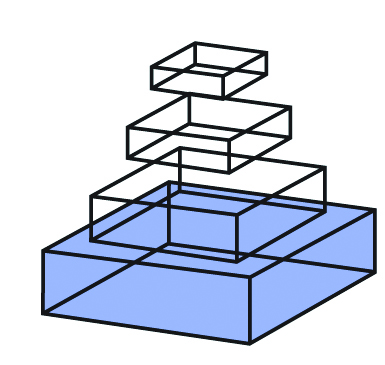
\includegraphics[width=3.5cm]{logo1}% This is a *.jpg file
%\end{center}
% \textbf{\refstepcounter{figure}\label{fig:01} Figure \arabic{figure}.}{ Enter the caption for your figure here.  Repeat as  necessary for each of your figures }
%\end{figure}

%\begin{figure}
%\begin{center}
%
\includegraphics[width=3.5cm]{logo2}% This is an *.eps file
%\end{center}
% \textbf{\refstepcounter{figure}\label{fig:02} Figure \arabic{figure}.}{ Enter the caption for your figure here.  Repeat as  necessary for each of your figures }
%\end{figure}

%%% Frontiers will add the figures at the end of the provisional pdf automatically %%%

%%% The use of LaTeX coding to draw Diagrams/Figures/Structures should be avoided. They should be external callouts including graphics.

\end{document}
